
\section{Introduction}

The primary purpose of the Developer's Guide is to provide the high-level
OO design and description of the C++ interfaces and concrete implementations
for the solution of a broad class of transient ordinary differential
equations (ODEs) and differential algebraic equations (DAEs) in a
consistent manner. Although Doxygen is a good tool to explore the
details of the C++ interfaces and classes, it rarely provides the
high-level interaction of these objects and how they are intended
to be used. Therefore in this Developer's Guide, the high-level description
is given in order for new Rythmos developers can get the basic design
of Rythmos. It is intended that this description should remain fairly
stable over time, and not require many updates. However detailed information,
which could change more often, is left to the Doxygen webpages, which
obviously provides quick and easy document generation of software
implementation.

\begin{figure}
\centering{}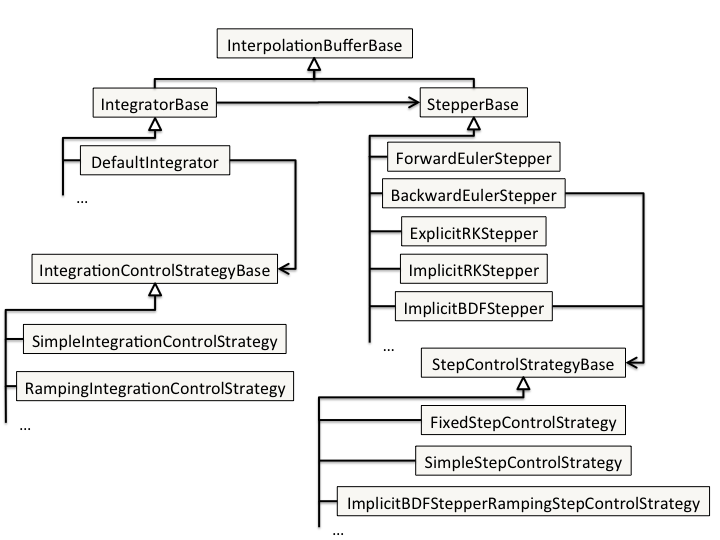
\includegraphics[width=5in]{figures/IntegratorStepperDesign}\caption{General relationships between the Integrators, IntegrationControlStrategies,
Steppers and StepControlStrategies.\label{rythmos:fig:IntegratorStepperDesign}}
\end{figure}



\subsection{Interpolation-Buffer Base\label{rythmos:sec:InterpolationBufferBase}}

An InterpolationBuffer is basically a container of solutions and time
derivatives (``states'') at discrete times (``time nodes'') over
a time range in ascending order, and can be used for storing checkpoints
and breakpoints of the state for later use. With an Interpolator specified,
a state at desired ``time points'' can be returned over the time
range with an accuracy of the order of the Interpolator. See Fig~\ref{rythmos:fig:InterpolationBuffer}.
\begin{figure}


\begin{centering}
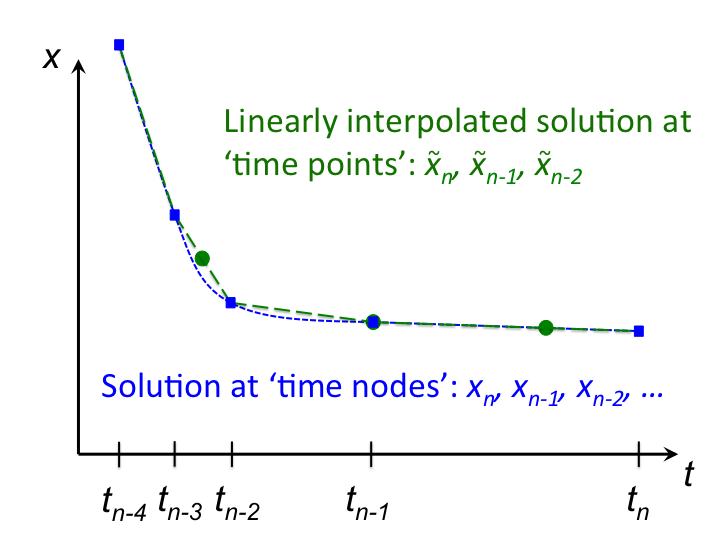
\includegraphics[width=4in]{figures/InterpolationBuffer}\caption{Illustrating the time points and time nodes in InterpolationBuffer
with a linear interpolator.\label{rythmos:fig:InterpolationBuffer}}

\par\end{centering}

\end{figure}


Part of the design here is to separate the state information (solutions
and time derivatives) from how the state is integrated to that time.
This can be used when separate ODEs and DAEs with different time integrators
are advanced in time, and wish to share their states (e.g., forward
and adjoint states, and operator-split solutions). No direct synchronizing
of time steps is required between them; time steps of each state can
be interpolated between for each integrator. 

An important caveat here is that the interpolated solutions are not
guaranteed to satisfy the ODE/DAE at the interpolated ``time points''.
This may be important for simulations where conservation is required,
e.g., conservation of mass, momentum and energy. The InterpolationBuffer
can be still useful in this situation, but the ``time nodes'' should
be used to ensure that the state satisfies the governing ODEs/DAEs.


\subsection{Integrator Base}

Time integration is carried out by Integrators, which inherit from
InterpolationBufferBase, and advance the state in time (step-by-step)
with Steppers. Integrators therefore have a set of states at given
times (see Sec.~\ref{rythmos:sec:InterpolationBufferBase}), and
can provide states to client requests. If the client requests a time
point within the current time range, the Integrator can simply return
an interpolated state. If the client requests a point forward in time,
the Integrator will advance the state to include the requested time.

The primary function of the Integrator is to manage the ``high-level''
time coordination required by the clients. Examples of this time marching
would include output of the solution state at various times, managing
checkpoints between solution states and adjoint states, coordinating
states between operator-split solutions, etc. All these coordinations
have very little to do with individual time steps, and more with times
where the solution states are required. This helps define the difference
between Integrators and Steppers when it comes to step-size selection
(Integration and Step Control Strategies).

In general the Integrator will request the largest step size required
to meet the next ``coordination'' (see Section~\ref{rythmos:sec:Integration-Control-Strategy}),
and leave the leave final determination of the step size to the Stepper
based on client specification, e.g., fixed or variable step size,
order, and accuracy (see Section~\ref{rythmos:sec:Step-Control-Strategy}).
Many times the step size completed by the Stepper will not advance
the state to the Integrator requested time, and the Integrator will
simply request another time step from the Stepper. With that said,
the Integrator has the flexibility to more directly control the time
stepping, and control the step size used by the Steppers. However
allowing the Stepper to choose the step size based on the Step Control
Strategy and having the Integration Control Strategy select ``coordination''
times is the preferred approach.


\subsection{Integration Control-Strategy\label{rythmos:sec:Integration-Control-Strategy}}

The Integration Control-Strategy is meant to determine the step size
needed for ``high-level'' simulation coordination (e.g., operator
splitting), solution output, and/or Stepper failure. In the Integration
Control-Strategy, we are not concerned with the accuracy of the solution,
as much as we are concerned with when are solutions needed. Obviously
one could control the Stepper step size with the Integration control-strategy
by using a \emph{fixed} step type and requiring the desired step size
be taken. This is especially useful for Steppers that can only handle
\emph{fixed} step types.


\subsection{Stepper Base}

A Stepper is a basic building block for DAE/ODE solvers. It advances
the state by ONE time step,
\[
x_{n-1}\underset{\Delta t}{\longrightarrow}x_{n},
\]
that has been requested by the Integrator. This time step can be fixed
or variable, where a \emph{fixed }step size indicates the stepper
will take the requested step size or fail, and where a \emph{variable}
step size allows the Stepper to adjust the step size to meet accuracy
and/or order requirements, and report to the Integrator the step size
taken. Most Steppers can be implemented very quickly for fixed step
sizes, and allow the Integrator to control the step size through an
Integration Control-Strategy (see Sec.~\ref{rythmos:sec:Integration-Control-Strategy}).
For variable step sizes, the Stepper needs a Step Control-Strategy
(see Sec.~\ref{rythmos:sec:Step-Control-Strategy}) in order to adjust
the step size based on error/order, and handle time step failures.


\subsection{Step Control-Strategy\label{rythmos:sec:Step-Control-Strategy}}

\begin{figure}
\centering{}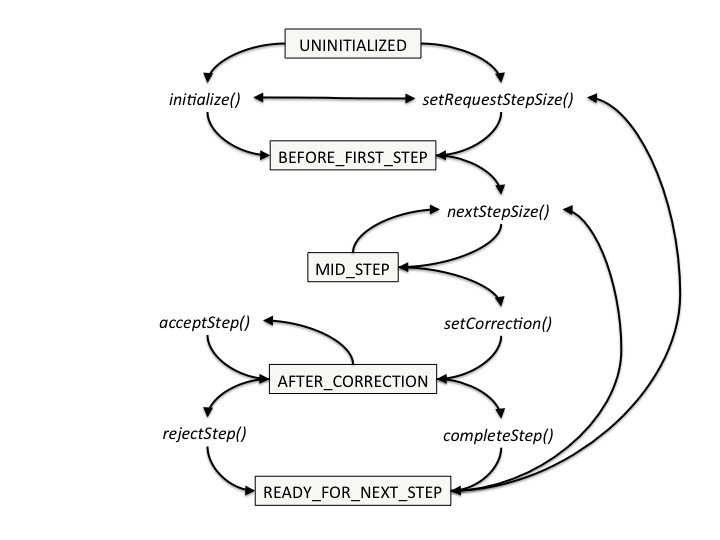
\includegraphics[width=5in]{figures/StepControlStrategy}\caption{Progression of the ControlStrategyState through a sequence of StepControlStrategy
functions by a Stepper.\label{rythmos:fig:StepControlStateProgression}}
\end{figure}
Step Control-Strategies are for adjusting the step size when a Stepper
is requested to take a variable step size by an Integrator. In order
to handle the correct progression of calls to Step Control-Strategies
functions (see Fig.~\ref{rythmos:fig:StepControlStateProgression}),
a ControlStrategyState is used, and can have the following values,
\texttt{\textsc{UNINITIALIZED}}, \texttt{\textsc{BEFORE\_FIRST\_STEP}},
\texttt{\textsc{MID\_STEP}}, \texttt{\textsc{AFTER\_CORRECTION}},
and \texttt{\textsc{READY\_FOR\_NEXT STEP}}.

The functions \emph{initialize()} and \emph{setRequestedStepsize()}
are used to prepare for the first step each time the Integrator calls
the Stepper, i.e., setting the requested step size and initializing
the Error Weight Vector. The \emph{nextStepsize() }function is used
to complete anything before starting the step. The \emph{setCorrection()}
functions is used to perform anything after the solver. i.e., the
correction. At this point the Stepper uses the StepControlStrategy
to determine if the step was acceptable with \emph{acceptStep(). }If
the step was acceptable, final computations of the solution and time
derivative are completed for the next time step by \emph{completeStep()}.
If the step was not acceptable, the step size and/order could be adjusted
by the StepControlStrategy function, \emph{rejectStep()}, and the
time step retried in order to obtain an acceptable time step. The\emph{
rejectStep()} function could completely reject the step and return
control to the Integrator to see if the Integrator Control Strategy
can do something to revive the time step.
